\documentclass[a4paper, 12pt,oneside]{article} 
%\documentclass[a4paper, 12pt,oneside,draft]{article} 
\usepackage{preamble}
%--------------------- ACTUAL FILE ---------------------- %
\begin{document} 
%%%
	\begin{center}
	    \Large
	    \textbf{Coin-Data Regression Study}\\
	    %\vspace{0.4cm}
		%\newline
	    \large
		Regression Methods Project \\
	    By Rayan Harfouche \& Tara Fjellman \\
	    \small{Fall 2024}
	\end{center}
	\section{Introduction}
	\begin{itemize}
		\item unbalanced dataset 
		\item number of people and coins
		\item few people with many coins and few coins with many people
		\item inspection of same side rates show sign of possible person, coin and person-coin dependence
		\item Learning effects investigated 
	\end{itemize}


	\section{Analysis}
		\subsection{Model Comparison}
			In this section, we introduce and compare different models for the same side success rate. 

			Some GLMs with binomial responses and some WLS ones based on the ... approximation.
			
			Should explain no a priori response transformation ...
			
			For each, the considered formulas in terms of the covariates are:
			\begin{itemize}
				\item \texttt{1}, corresponding to a constant model.
				\item \texttt{1+C(person)}, corresponding to a model with the person as a covariate.
				\item \texttt{1+C(person)+C(coin)}, corresponding to a model with the person and the coin as covariates.
				\item \texttt{1+C(person)+C(coin)+C(person):C(coin)}, corresponding to a model with the person, the coin, and the interaction between the person and the coin as covariates.
			\end{itemize}
			* model 4 could seem redundant due to nesting-main effect, but we ....
			*  

			Should explain why eliminated some covariates ...
			\subsubsection{WLS Approach}

			\subsubsection{GLM Approach}
			\lipsum[1]
			\begin{table}[htb]
				\centering
				\caption{Model comparison for different models.}
				\label{tab:model-comparison}
				\begin{tabular}{lccc}
				\toprule
				Model & Deviance & AIC & Model DF \\
				\midrule
				\texttt{1} & 3943.48 & 173.97 & 0 \\
				\texttt{1+C(person)} & 3677.51 & 0.00 & 46 \\
				\texttt{1+C(person)+C(coin)} & 3611.12 & 17.61 & 88 \\
				\bottomrule
				\end{tabular}
			\end{table}
			\lipsum[1]
			\begin{figure}[htb]
				\centering
				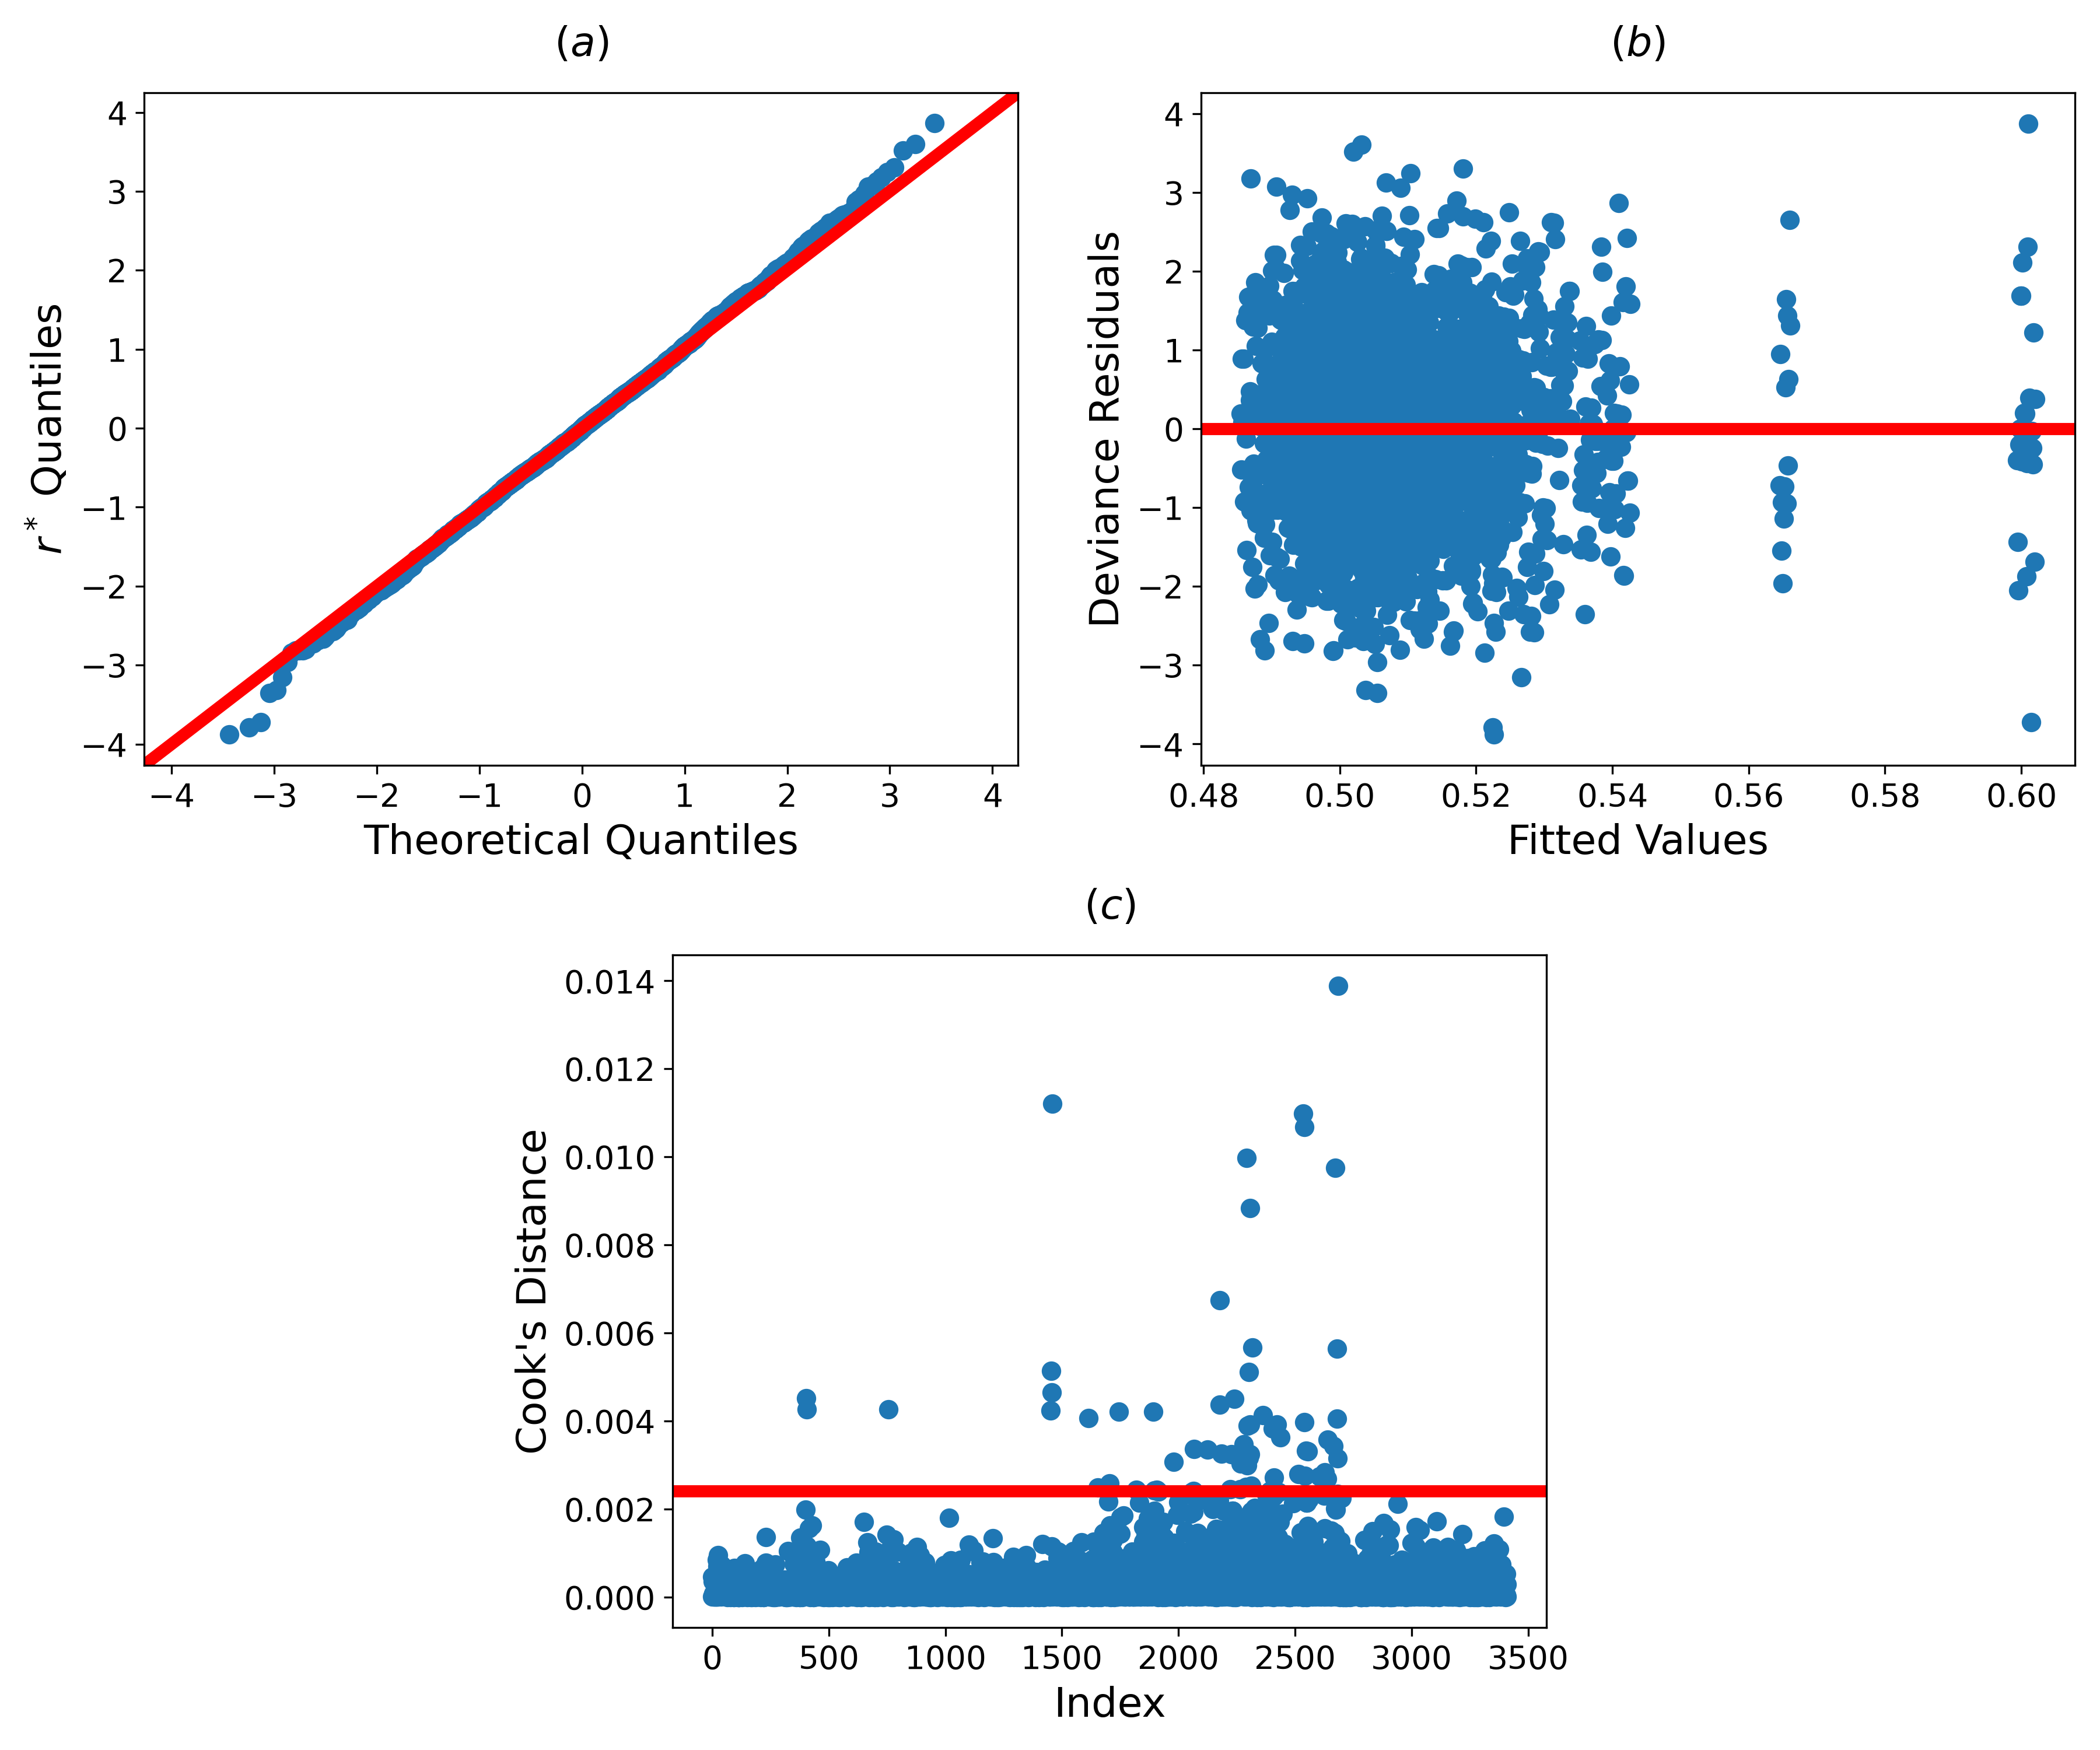
\includegraphics[width=0.85\textwidth]{GLM_diagnostics.png}
				\caption{Diagnostics for the selected GLM model. (a).}
				\label{fig:glm-diagnostic}
			\end{figure}
			\lipsum[1]
			\begin{table}[htb]
				\centering
				\caption{Likelihood ratio tests between models.}
				\label{tab:llr-comparison}
				\begin{tabular}{llc}
				\toprule
				Tested model & Restricted model & $p$-value \\
				\midrule
				\texttt{1+C(person)} & \texttt{1} & 0.00e+00 \\
				\texttt{1+C(person)+C(coin)} & \texttt{1+C(person)} & 9.61e-03 \\
				\bottomrule
				\end{tabular}
			\end{table}
		\subsection{Unusual Observations}
		\begin{figure}[htb]
			\centering
			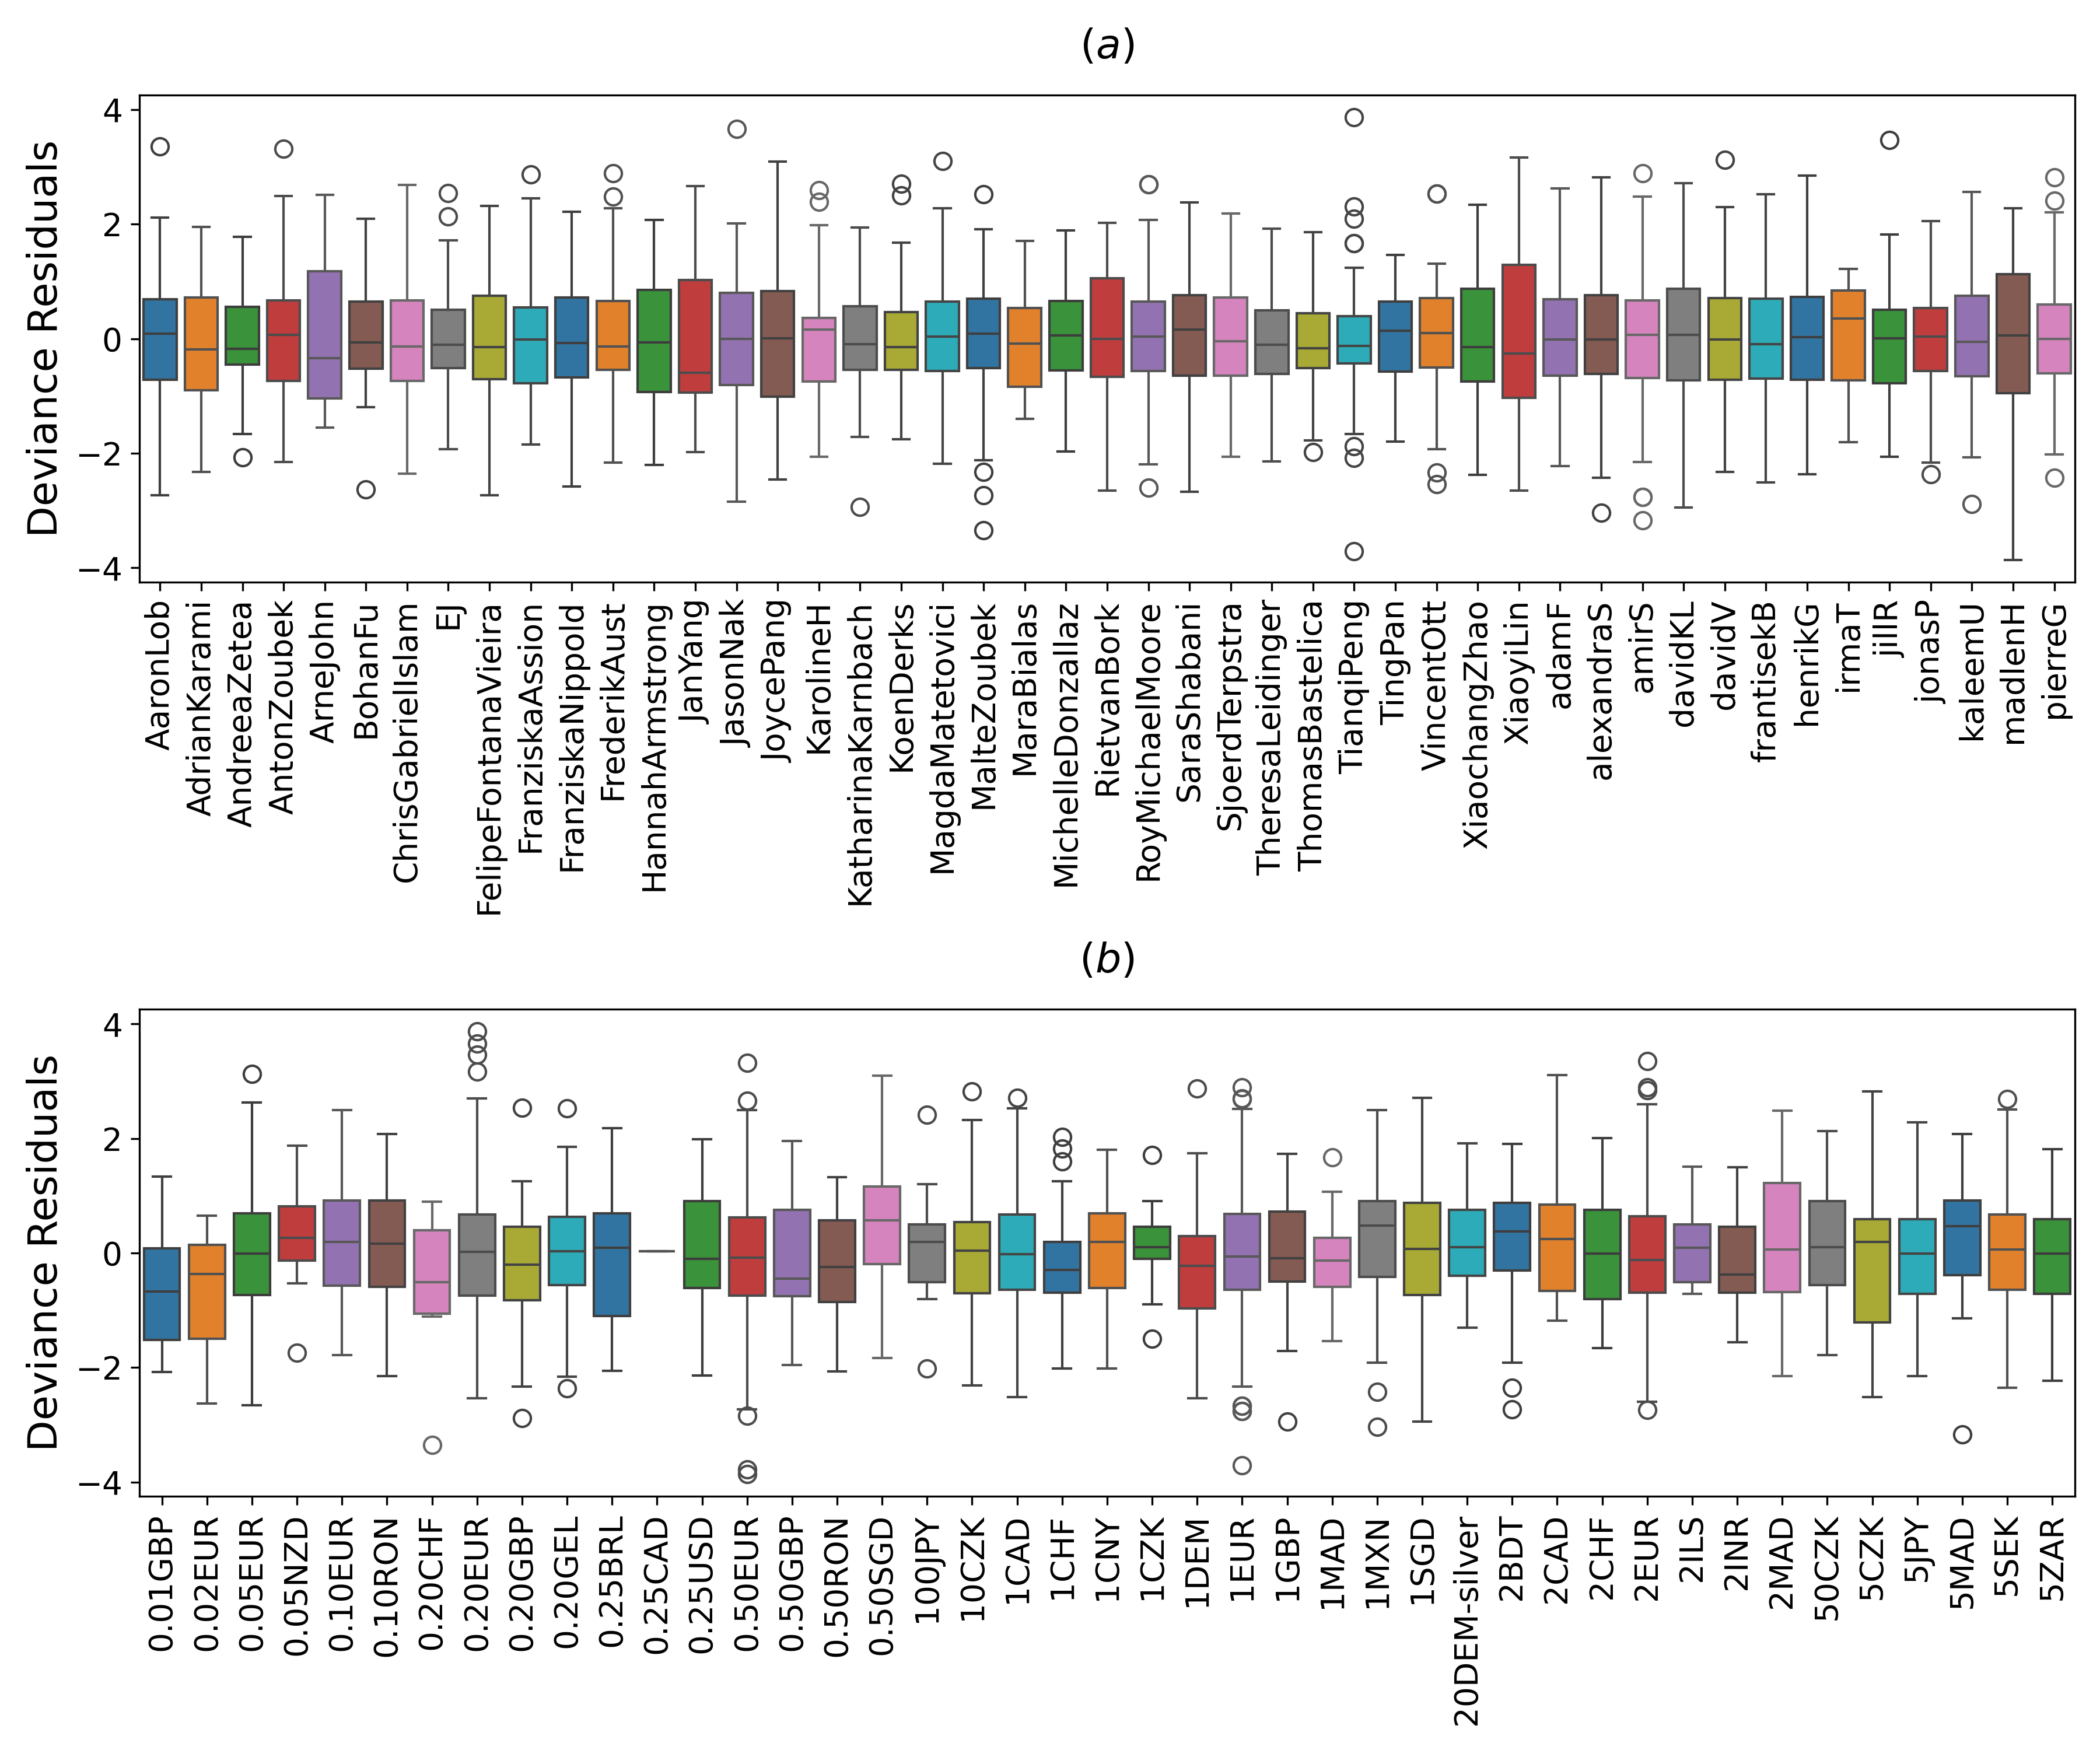
\includegraphics[width=0.85\textwidth]{dev_resid_vs_covariates.png}
			\caption{Dev-resid as a function of (a) person and (b) coin.}
			\label{fig:dev-resid-vs-covariates}
		\end{figure}

		\subsection{Learning Effects}
		\lipsum[1]
		\begin{figure}[htb]
			\centering
			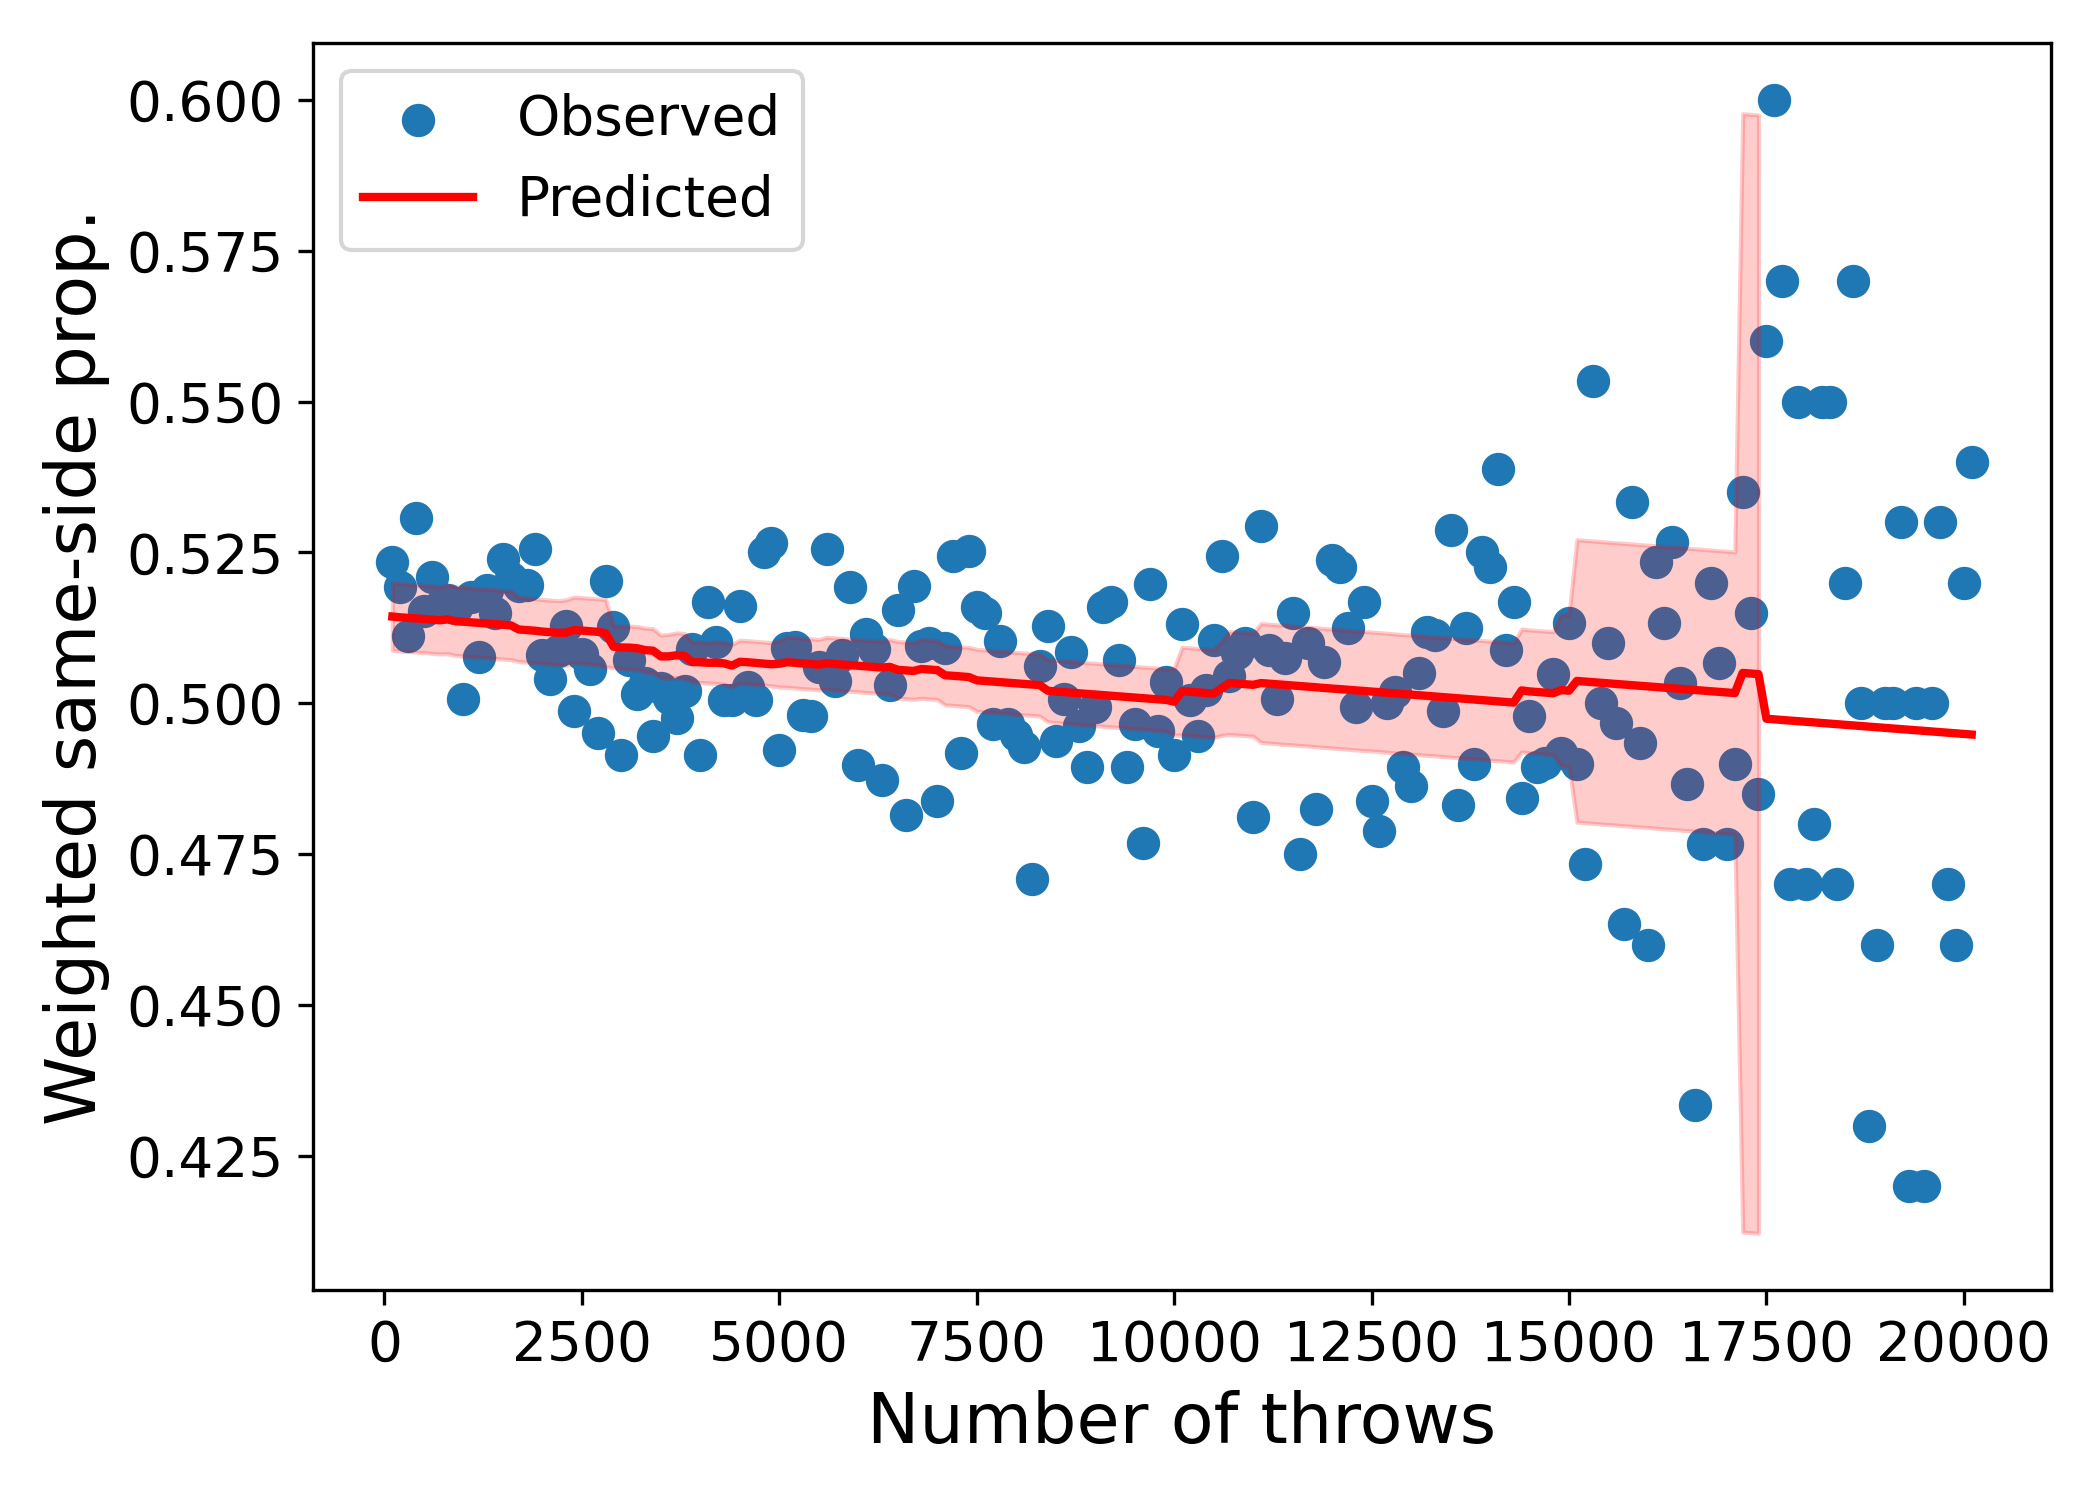
\includegraphics[width=0.5\textwidth]{learning_effects.png}
			\caption{Learning effects.}
			\label{fig:learning-effects}
		\end{figure}
		\subsection{Memory Effects ??}

	\section{Discussion}
	\section{Conclusion}
	\section*{Acknowledgements}
	\section*{References}
	%\appendix
	%	\section{Runtime Estimation}\label{appendix:runtime_estimation}
%%%
\end{document} 